\documentclass[12pt,a4paper]{scrartcl}		% KOMA-Klassen benutzen!

%\usepackage[ngerman]{babel}			% deutsche Namen/Umlaute
\usepackage[utf8]{inputenc}			% Zeichensatzkodierung
\usepackage{url}
\usepackage{graphicx}
\usepackage{amsmath}
\usepackage{multicol}
\usepackage{glossaries}
\usepackage{expdlist}
\usepackage{subfig}
\usepackage{listings}
% see http://tex.stackexchange.com/questions/35145/maintaining-layout-of-tikz-diagrams-with-tex4ht-converting-as-single-pictures
\ifx\HCode\UnDef\else\def\pgfsysdriver{pgfsys-tex4ht.def}\fi
\usepackage{tikz}
  \usetikzlibrary{positioning,arrows,fit}
  \usetikzlibrary{decorations.pathmorphing,backgrounds,fit,decorations.pathreplacing}

\usepackage{setspace} % Anderthalbfacher Zeilenabstand ist Standard in den meisten Seminararbeiten. Das Paket setspace ermöglicht ein einfaches Umstellen von normalem, anderthalbfachen oder sogar doppeltem Zeilenabstand. 
\usepackage[paper=a4paper,inner=25mm,outer=20mm,top=15mm,bottom=20mm]{geometry} %Das geometry Paket dient zur Einrichtung der Seiten. Hier werden die jeweiligen Seitenränder angegeben. Diese wWerte sollten durch die jeweiligen Vorgaben des Seminarleiters oder Instituts ersetzt werden.
\setlength{\parindent}{1.7em} %Neue Abschnitte werden mit hängendem Einzug gesetzt, parindent definiert. um wie viel der Absat eingerückt wird. Die Einheit em ist abhängig vom verwendeten Zeichensatz und daher absoluten Werten in mm oder cm vorzuziehen. 
\setcounter{secnumdepth}{3} %Bis zu welcher Gliederungsebene nummeriert werden soll gibt dieser Befehl vor. In Falle 3 werden \section, \subsection und \subsubsection nummereiert.
\setcounter{tocdepth}{2} %Bis zu welcher Ebene Einträge ins Inhaltsverzeichnis aufgenommen werden. In diesem Beispiel ebenfalls bis Ebene drei (\subsubsection). Ein durch \paragraph ausgewiesener Abschnitt wird demnach nicht im Inhaltsverzeichnis auftauchen. 

\usepackage[colorlinks=false, pdfborder={0 0 0}, plainpages=false]{hyperref}

% http://tex.stackexchange.com/questions/9497/start-new-page-with-each-section
\usepackage{titlesec}
\newcommand{\sectionbreak}{\clearpage}

\usepackage{tocbibind}

\newcommand{\citeurl}[2]{\url{#1} (#2)}

\begin{document}
\lstnewenvironment{javalisting}[1][]
  {\lstset{language=Java,float=tb,#1}}% \begin{javalisting}[...]
  {} % \end{javalisting}

\lstnewenvironment{anylisting}[1][]
  {\lstset{float=tb,#1}}% \begin{anylisting}[...]
  {} % \end{anylisting}

\lstset{ %
  language=Java,
  float=tb,
  frame=single,
  captionpos=b
}

%\titlehead{}
%\subject{subject}
\title{}
\subtitle{}
\author{Thomas Koch\\\url{thomas@koch.ro}\\matriculation number 7250371}
\publishers{Fernuniversität Hagen\\Faculty of mathematics and computer science}
\date{\today}
%\thanks{}
\maketitle{}

%\newpage{}
\tableofcontents{}
\begin{abstract}

\end{abstract}
\newpage{}

\section{Introduction}

Although computers became ubiquitous for some time now, they still don't help
their users with their most basic information management needs: Make contacts,
calendars, notices and to do items available across different devices and share
them with family and peers.

Most existing solutions are either based on non-free software (Microsoft Outlook),
or require the user to trust his personal data to the commercial
interests of a multinational corporation.
%\footnote{Experiences with Android and Data in the cloud \citeurl{http://keithp.com/blogs/calypso}{?}}

% @TODO Überleitung

A section about OpenSocial (\autoref{sec:opensocial}) provides additional
motivation for a restful API for social data. It also uses the opportunity to
provide an alternative approach to explain the rest architecture by going into
detail why OpenSocial is not restful.

A few patterns or techniques are presented and proposed for reuse in other Rest
applications to ease the support for multiple alternative Media types. Among
these techniques are Dependency Injection to prepare resource method parameters
(\autoref{sec:prep-requ-comp}), Resource Facades
  (\autoref{sec:resourcefacades}) and a programmable dispatcher
  (\autoref{sec:dispatcher}).

\subsection{Definitions}
%@TODO
Kolab is the name of a software product ... TODO

A couple of related terms and concepts exist that all more or less overlap with
the functionality provided by Kolab: Groupware, Personal Information
Management/Manager (PIM), Group Information Management (GIM), Computer-supported
cooperative/collaborative work, Knowledge management, (Enterprise) Content
Management. For the rest of this work a Groupware is a software managing address
books, calendars, todo items, journals and probably more data for a group of
collaborating users.

\subsection{Related work}
\subsubsection{WebDAV, CalDAV, CardDAV}

The most widely implemented Groupware protocols (in free software) today seem to
be CalDAV\cite{RFC4791} for calendaring and CardDAV\cite{RFC6352} for
contacts\footnote{only full free server implementations: Apple Calendar Server,
  Bedeworks, DAViCal, eGroupWare, Owncloud, SOGo}. Both protocols extend
WebDAV\cite{RFC4918} and thus inherit its characteristics.

Two characteristics of WebDAV motivate an investigation of alternative
approaches. The first is the protocol's complexity that complicates correct
implementation. Unfortunately complexity is hard to assess. Therefor only some
indications are provided at this point.

Lisa Dusseault, author of a WebDAV book\cite{Dusseault2004} and the standard
itself
wrote\footnote{\citeurl{http://nih.blogspot.com/2008/02/nearly-two-years-ago-i-made-prediction.html}{2012-1-6}}:

\begin{quote}
Were I to propose CalDAV today it would probably be CalAtom.
\end{quote}

The three standards WebDAV (127p), CalDAV (107p) and CardDAV (48p) add up to 282
pages of highly specific standards. This is nearly double as much text as
necessary for the standards this work is based on (149 pages)\footnote{Atom (43),
  AtomPub (53), Feed paging (15), OpenSearch (~28), Atom Deleted Entry (10)}. In
contrast to WebDAV, Feeds and related technologies are also widely used so that
a web developer might already know the latter standards.

The second and for this work more important characteristic of WebDAV is, that it
is not restful, as explained by Roy
Fielding:\footnote{\citeurl{http://tech.groups.yahoo.com/group/rest-discuss/message/5874}{2012-3-5}}

\begin{quotation}
  PROP* methods conflict with REST because they prevent important resources from
  having URIs and effectively double the number of methods for no good
  reason. [\ldots] It really doesn't matter how uniform they are because they
  break other aspects of the overall model, leading to further complications in
  versioning (WebDAV versioning is hopelessly complicated), access control
  (WebDAV ACLs are completely wrong for HTTP), and just about every other
  extension to WebDAV that has been proposed.

  [\ldots]

  The problem with MOVE is that it is actually an operation on two independent
  namespaces (the source collection and destination collection). The user must
  have permission to remove from the source collection and add to the
  destination collection, which can be a bit of a problem if they are in
  different authentication realms. COPY has a similar problem, but at least in
  that case only one namespace is modified. I don't think either of them map
  very well to HTTP.
\end{quotation}

% \url{http://microformats.org/discuss/mail/microformats-rest/2006-April/thread.html#217}
% see \cite{Amundsen2010} for a restful approach to properties.
% \begin{quote}
%   AtomPub is different from DAV in two key respects:
%   \begin{itemize}
%   \item The client doesn't control where things go, the server does
%   \item It is allowed and expected that an AtomPub server will look at the incoming information and change it (generate ID, timestamps, sanitize HTML, etc)
%   \end{itemize}
% \end{quote}
% Tim Bray, http://www.imc.org/atom-protocol/mail-archive/msg11271.html

Given the comprehensiveness of CalDAV and CardDAV one would expect these
protocols to cover all common use cases. However the calconnect consortium
additionally develops two alternative protocols, CalWS-SOAP and
CalWS-REST\footnote{\citeurl{http://calconnect.org/CD1012_Intro_Calendaring_V1.1.shtml}{2012-3-5}}.

\subsubsection{IMAP used by Kolab}

The Kolab Groupware Server is special in that it uses the Internet Message
Access Protocol (IMAP) as a synchronization protocol for all its data and thus
the IMAP server as a database.

There are a few appealing advantages to this approach:

\begin{itemize}
  \item The IMAP infrastructure used for mail can be reused.
  \item Data is stored as file attachment. Thus the probably complicate mapping of
  groupware data items to the needs of a (relational) database is avoided.
  \item IMAP already supports offline work and later synchronization.
\end{itemize}

The simplicity of just dropping files in a store used by several concurrent
clients however also has drawbacks, e.g: there is no moderating logic on the
server site that could verify the correctness of stored data and there are no
query capabilities.

IMAP in general also comes with its own challenges:

\begin{itemize}
\item The standard documents describing and extending IMAP are
  many\footnote{\citeurl{http://www.apps.ietf.org/rfc/ipoplist.html}{2012-3-5}}.
\item IMAP imposes a folder structure and does not permit alternative structures
  like tags as used by Google's gmail.
\item Sam Varshavchik, author of the Courier Mail Transfer Agent, argues that
  IMAP standard documents are ``contradictory'' and that implementations define
  their own understanding of what IMAP
  is\footnote{\citeurl{http://www.courier-mta.org/fud}{2012-3-5}}.
\end{itemize}

% \item Some attempts to create a simpler alternative to IMAP:
%   \begin{itemize}
%   \item http://en.wikipedia.org/wiki/POP4
%   \item \url{http://en.wikipedia.org/wiki/Simple_Mail_Access_Protocol} also here http://www.courier-mta.org/cone/smap1.html
%   \item \url{http://en.wikipedia.org/wiki/Internet_Mail_2000}
%   \item HTTP restful: http://tools.ietf.org/id/draft-dusseault-httpmail-00.txt mailing list: https://www.ietf.org/mailman/listinfo/httpmail
%   \item BikINI is not IMAP http://bikini.caterva.org
%   \item Outlook uses HTTP to communicate with Hotmail
%   \item another rest mail proposal: http://www.prescod.net/rest/restmail/
%   \end{itemize}
% \item more rants: http://blog.gaborcselle.com/2010/02/how-to-replace-imap.html
% \item IMAP issues found by the chandler project http://chandlerproject.org/bin/view/Jungle/IntrinsicIMAPIssues

\subsubsection{OpenSocial, useful but not restful}
\label{sec:opensocial}

OpenSocial\cite{OSSpec2.0.1} specifies how data of social networks can be
accessed by clients, especially Javascript browser widgets. While the
specification was initially designed for social networks, it has also been
adopted to enhance wikis, issue trackers (Confluence, Jira from Atlassian),
Groupware (Lotus from IBM), Content Management Systems (Alfresco,
Nuxeo). \cite{Huebner2009} discusses the benefits of OpenSocial for the
interaction of university members.

The specification is discussed in this section because it shows the usefulness
of making social data available for different kind of clients but on the other
hand is a poster child for a non-restful API on top of HTTP and thus serves as a
standard of comparison for the API to be designed in this work.

Restful APIs are modeled around resources, their representations and links
between them\cite[sec. 5.1.5]{Fielding2000}\footnote{ ``REST is defined by four
  interface constraints: identification of resources; manipulation of resources
  through representations; self-descriptive messages; and, hypermedia as the
  engine of application state.''}. The authors of OpenSocial however seem to
have started already from a different concept\cite[Social API Server, sec 2,
Services]{OSSpec2.0.1}:
\begin{quote}
  OpenSocial defines several services for providing access to a container's data.
\end{quote}

Fielding wrote a blog post stating that OpenSocial\footnote{Fielding referred to
  a concrete implementation, the ``SocialSite REST API''.} would not be
restful\cite{Fielding2008}. He pointed out rules ``most often violated within
so-called REST APIs'', but did not give explicit examples, how OpenSocial
violates them.

\begin{quote}
  A REST API should not be dependent on any single communication protocol,
  [\ldots] any protocol element that uses a URI for identification must allow
  any URI scheme to be used for the sake of that identification.
  \textit{[Failure here implies that identification is not separated from
    interaction.]}
\end{quote}

OpenSocial defines a construct called ``REST-URI-Fragment'' which is a clear
violation of the above rule. This URI fragment is simply an encoding of
procedural parameters as elements of an HTTP URI:\cite[Core API Server, sec
2.1.1.2.2, REST-URI-Fragment]{OSSpec2.0.1}

\begin{quote}
  Each service type defines an associated partial URI format. The base URI for
  each service is found in the URI element associated with the service in the
  discovery document. Each service type accepts parameters via the URL
  path. Definitions are of the form:
  
  \verb:{a}/{b}/{c}:
\end{quote}

URIs can contain a query component that would be more appropriate to contain
parameters. This would also have made it clearer to see that the specification
actually defines services instead of resources. One test showing the misfit is
to ask how dot-segments ('.' and '..') inside the URI fragment are interpreted
and whether this conforms with the letter and spirit of the URI
standard\cite[sec 3.3]{RFC3986}. Another misfit can be seen in the URI fragment
to retrieve one or multiple albums. In this case the 'c' part in the quoted
definition above is actually a list of albums to retrieve separated by a slash.

Fielding's second bullet point most likely refers to the
\texttt{X-HTTP-Method-Override} header. This header is a widely
used\footnote{\citeurl{http://www.subbu.org/blog/2008/07/another-rest-anti-pattern}{2011-12-06}}
workaround to allow the use of other HTTP methods than GET and POST from HTML
forms or through firewalls.

The next two points again refer to a more serious issue:

\begin{quote}
  A REST API should spend almost all of its descriptive effort in defining the
  media type(s) used for representing resources and driving application
  state[\ldots].  \textit{[Failure here implies that out-of-band information is
    driving interaction instead of hypertext.]}  A REST API must not define
  fixed resource names or hierarchies[\ldots] \textit{[Failure here implies that
    clients are assuming a resource structure due to out-of band
    information[\ldots]].}
\end{quote}

The OpenSocial specification contains a lot of out-of-band information
describing how to form URIs to access information or which methods to use on
which URIs for different actions. This means that the OpenSocial API is not
simple or intuitive to use but requires a client developer to read a lot of
specification, thus violating the simplicity property of a restful
architecture. Since the URIs are fixed in the specification and necessarily also
in clients, the modifiability property is also violated\cite[sec
2.3]{Fielding2000}.

The following tables give some examples of the specified URIs:

\begin{table}[h]
\begin{tabular}{p{6.5cm} l p{10cm}}
  URI fragment & Method & Description \\
  %\hline
  \verb:/people/{User-Id}/@self: & GET & profile for User-Id \\
  \verb:/people/{User-Id}/@self: & DELETE & remove User \\
  \verb:/people/{User-Id}/{Group-Id}: & GET & full profiles of group members \\
  \verb:: & POST & Create relationship, target specified \newline by \verb:<entry><id>: in body \\
   & POST & Update Person \\
  \verb:/people/{Initial-User-Id}/: \newline \verb:{Group-Id}/{Related-User-Id}: & GET & ??? \\
  \verb:/people/@supportedFields: & GET & list of supported person profile fields \\
  \verb:/groups/{User-Id}[/{Group-Id}]: & GET & one or all groups of a user \\
   & PUT & update group \\
   & DELETE & delete group \\
  \verb:/groups/{User-Id}: & POST & create group \\
\end{tabular}
  \caption{URI fragments for peoples and groups in the OpenSocial REST API}
\end{table}

\begin{table}[h]
\begin{tabular}{p{9.5cm} l p{8cm}}
  URI fragment & Method & Description \\
  %\hline
  \verb:/albums/{User-Id}/@self: & POST & create album \\
  \verb:/albums/{User-Id}/{Group-Id}[/Album-Id]*: & GET & one or multiple albums \\
  \verb:/mediaItems/{User-Id}/{Group-Id}/{Album-Id}/: \newline \verb:{MediaItem-Id}: & GET & one mediaitem \\
  \verb:/mediaItem/{User-Id}/@self/{Album-Id}: (sic!) & POST & create mediaitem \\
\end{tabular}
  \caption{URI fragments for albums and mediaitems in the OpenSocial REST API}
  \label{tab:OSURIAlbums}
\end{table}

The last URI in \autoref{tab:OSURIAlbums} is obviously missing an ``s'' behind
\texttt{mediaItem}. This typo is present and unfixed in the OpenSocial spec
since Version 1.0, released in march 2010. This is of course not a big issue in
itself, but rather a sign that the specification is too verbose and does
over-specify things that should rather be auto-discovered through hyperlinks.

Fielding mentions in a comment to the same blog post that the OpenSocial API
``could be made so [restful] with some relatively small changes'' but does not
specify these changes. However some issues can easily be identified.

First the data structures defined in OpenSocial do not use URIs to refer to
other resources. Instead they use Object-Ids that must then be inserted in the
appropriate URI templates. Examples are the \texttt{recipients},
\texttt{senderId}, \texttt{collectionIds} of messages and the \texttt{ownerId}
of albums. The person structure does not contain fields referencing other
resources. Thus it does not obviously violate REST like the albums and
messages. However it does so even worse since there are hidden references only
defined out-of-band in the specification. One can retrieve the albums, relations
or messages of a user by filling in the \texttt{userId} in one of the specified
URI templates. If Users would just contain references to other resources related
to a user, the specification could already be shortened a lot.

Another missed opportunity for a much more intuitive API is the relation of
media items and albums. This seems to be poster child example for a collection
(album) to collection-element (media item) relation which could have made use of
the hierarchical character of URI paths. OpenSocial however requires the client
developer to use two different URI templates. (\autoref{tab:OSURIAlbums})

A not so small change to OpenSocial would be to either use already standardized
and registered media types where possible or to register new types where
necessary. It seems that there are some already existing media types that could
be a good fit for OpenSocial but only miss a canonical json representation for
easy consumption by javascript applications. These are vCard for
persons,\footnote{OpenSocial persons are based on portable contacts which in
  turn borrowed field names from vCards.} ATOM entries\cite{RFC4287} for
messages, activities and media items and ATOM categories, collections or
workspaces\cite{RFC5023} for albums and groups. It would probably be necessary
to add extensions to the mentioned media types but vCard and ATOM both already
anticipated this need and provided mechanisms to do so.

The use of the ATOM format could promote the adoption of OpenSocial because
developers could either reuse existing knowledge about ATOM or would be more
motivated to learn about a system that is based on an already widespread
format. In fact OpenSocial already mentions ATOM as a way to wrap OpenSocial
data. However this wrapping does not build extend and reuse ATOM semantics as
proposed above but just puts the OpenSocial data structures inside the
entry/content element of ATOM. This kind of misuse of ATOM does of course not
deliver any advantage on top of the existing plain JSON or XML
representations.\footnote{compare Bill de Hora, Extensions v Envelopes. 11/2009 
%\newline
  \citeurl{http://www.dehora.net/journal/2009/11/28/extensions-v-envelopes}{2011-21-07}}
Consequently the newest OpenSocial specification deprecates any reference to the
ATOM format.

In Jan Algermissen's ``Classification of HTTP-based
APIs''\footnote{\citeurl{http://nordsc.com/ext/classification_of_http_based_apis.html}{2011-12-08}},
the OpenSocial REST API would actually be ``HTTP-based Type I'' due to the lack
of media types and direct hyper links between related resources. Algermissen
writes that this level has the lowest possible initial cost of all HTTP APIs. Or
in other words: The OpenSocial specification authors might not have had to
invest a lot to come up with this API specification but maintenance and
evolution cost may be medium or high.

\subsubsection{Others}

The Calendar Access Protocol (CAP)\cite{RFC4324} was published in December 2005
about one year before CalDAV and CalAtom. The standard comprises 131 pages. No
evidence of any successful implementation could be found\footnote{One free
  implementation project \citeurl{http://opencap.sourceforge.net}{2012-3-5}
  seems inactive since 2005}. Cyrus Daboo, author of some calendaring standards,
attributes the failure of CAP to its
complexity\footnote{\citeurl{http://lists.calconnect.org/pipermail/caldeveloper-l/2012-January/000135.html}{2012-01-04}}.

CalAtom and CardAtom build on top of the Atom Publishing Protocol and are
therefor discussed in \autoref{sec:atom-publ-prot}.

The idea of using Feeds for collection synchronization has also been adapted by
Microsoft's
FeedSync\footnote{\citeurl{http://feedsyncsamples.codeplex.com}{2012-3-8}}. FeedSync's
most important contribution according to \cite{Snell2007} was the concept of a
``tombstone'' element to indicate the deletion of entries from a collection. An
RFC to standardize the tombstone concept\cite{draft-snell-atompub-tombstones-14}
for Atom feeds is currently in the late stages of the IETF standardization
process.
% http://notes.kateva.org/2008/01/microsoft-feedsync-what-heck-is-it-and.html

\section{Requirements}


% SRS template from http://code.google.com/p/e-bibliophile/wiki/SRS
%\subsection{Scope}
% This subsection should
% a)Identify the software product(s) to be produced by name (e.g., Host DBMS, 
% Report Generator, etc.);
% b)Explain what the software product(s) will, and, if necessary, will not do;
% c)Describe the application of the software being specified, including relevant 
% benefits, objectives, and goals;
% d)Be consistent with similar statements in higher level specifications 
% (e.g., the system requirements specification), if they exist.

\subsection{Scope and General Requirements}
% This subsection of the SRS should provide a summary of the major functions 
% that the software will perform. For example, an SRS for an accounting program 
% may use this part to address customer account maintenance, customer statement, 
% and invoice preparation without mentioning the vast amount of detail that each 
% of those functions requires.
% Sometimes the function summary that is necessary for this part can be taken 
% directly from the section of the higher level specification (if one exists) 
% that allocates particular functions to the software product. Note that for the 
% sake of clarity
% a)The functions should be organized in a way that makes the list of functions 
% understandable to the customer or to anyone else reading the document for the 
% first time.
% b)Textual or graphical methods can be used to show the different functions 
% and their relationships. Such a diagram is not intended to show a design of 
% a product, but simply shows the logical relationships among variables.

The software system designed in this work should provide a web based interface
for most common interactions with a Groupware system like Kolab. It must obey
the constraints of the REST architectural style\cite{Fielding2000}.

Guidelines of the design are:

\begin{itemize}
\item The system should be extensible to support different kind of personal
  information resources like contacts, events, todo items, journal items and
  free-busy informations.
  \item The CRUD operations must be supported: Create, Read, Update, Delete.
  \item The client must be able to synchronize collections of resources for
    offline read access and manipulation.
  \item The design should be considerably ``easier'' to implement then CalDAV,
    CardDAV or IMAP as well for the server as for the client.
  \item The design should reuse existing standards where possible.
  \item The design should support all client types listed in
    \autoref{sec:user-class-char}.
  \item The design should support different Media Type representations of
    resources.
\end{itemize}

% restful: one entry point, reuse of existing protocols and media types
% easy to understand and implement
% Collections z.B. für Projekte könnten alle möglichen Typen konsumieren.

\subsection{Replacement for CardDAV}
\label{sec:replacement-carddav}

The web application should provide at least the main features of the CardDAV
protocol. It should be demonstrated that a restful application can serve for the
same purpose and thus that the additional complexity of WebDAV and CardDAV may
not be necessary for most use cases.

The standard lists the main features of CardDAV\cite[sec. 1]{RFC6352}:

\begin{enumerate}
\item Ability to use multiple address books with hierarchical layout.
\item Ability to control access to individual address books and address entries
  as per WebDAV Access Control List (ACL) [RFC3744].
\item Principal collections can be used to enumerate and query other users on
  the system as per WebDAV ACL [RFC3744].
\item Server-side searching of address data, avoiding the need for clients to
  download an entire address book in order to do a quick address 'expansion'
  operation.
\item Well-defined internationalization support through WebDAV's use of XML.
\item Use of vCards [RFC2426] for well-defined address schema to enhance client
  interoperability.
\item Many limited clients (e.g., mobile devices) contain an HTTP stack that
  makes implementing WebDAV much easier than other protocols.
\end{enumerate}

There are some minor features of CardDAV, that are mainly inherited from WebDAV
and whose general usefulness outside of the scope of a content management system
could be argued. See \autoref{sec:excluded-requirements} for a discussion of
those.

\subsection{REST architectural style}

The requirement to obey the constraints of REST should cause the system to have
some characteristics that may be especially advantageous for the use case of a
Groupware API. Those characteristics are, according to \cite{Fielding2000}:

\begin{itemize}
\item Cacheability (sec. 5.1.4) can keep the data available also in offline
  mode, improves performance and scalability.
\item Simplicity (sec. 2.3.3) helps to integrate the Groupware with other
  applications, e.g. publishing birthdays of employees in an intranet portal.
\item Modifiability (sec. 2.3.4) allows to adapt the Groupware to changes in the
  organization.
\item Reliability (sec. 2.3.7) can be of great importance, if the ability to
  work depends on the correct working of the Groupware system.
\item Anarchic scalability (sec. 4.1.4.1) allows a Groupware to function with
  other components that are not under the control of the Groupware
  administrator.
\end{itemize}

% Other outcomes described by Fielding that may not be of importance for the
% present work are: scalability in terms of users, network performance and
% efficiency.

\subsection{User Classes and Characteristics}
\label{sec:user-class-char}

Different kinds of clients should be able to use the API.
\autoref{tab:clientsconstraints} lists clients whose constraints and
characteristics must be respected in the design. The choice of clients and their
characteristics is intentionally conservative to cover a wide range of real
world use cases.

\begin{table}[tbh]
  \centering
  \begin{tabular}[tbh]{ r || c | c | c | l }
                      & Memory & Bandwidth & preferred format & comment \\  \hline
  Web Browser (HTML5) &  5 MB & 56 kbit/s & JSON & workplace, internet cafe\\
  Mobile Device       &  512 MB & 384 kbit/s & any/XML & Smart Phone, Tabled \\ 
  Desktop application &  1 GB & 10 Mbit/s  & any/XML & PIM suite \\
  Server application  &  4 GB & 100 Mbit/s & any/XML/HTML & intranet application \\
  \end{tabular}
  \caption{Constraints of different API clients}
  \label{tab:clientsconstraints}
\end{table}

The most problematic client in the list is the web browser with only 5MB of
storage capacity (via
WebStorage\footnote{\citeurl{http://www.w3.org/TR/webstorage/}{2012-2-2}}) a
potentially very bad internet connection, the inability to leave data for later
sessions (internet cafe) and the restriction to one particular format
(JSON). However this use case is of importance as the
OpenSocial~(~\ref{sec:opensocial}) case shows. It is also the primary use case
to justify an API that provides multiple Media Types since it mandates JSON
while the canonical Media Types (xCard, xCal) support XML.

\subsection{Data Characteristics}
\label{sec:data-characteristics}

Lacking sources for more accurate numbers, a couple of conservative estimates
are made for the size and number of resources in the scope of this work. This
guesswork is not perfect. But it provides a rationale behind later design
decisions (\autoref{sec:interactions}) and outlines their applicability for a concrete use case.

\subparagraph{Contacts}

It is believed that humans have regular social contacts to around 150
people\footnote{\citeurl{http://en.wikipedia.org/wiki/Dunbar's_number}{2012-2-29}}. So
the number of contacts in a users address book collection should at least handle
1500 contacts.

The average textual data size associated to a contact is expected to be around
840 bytes\footnote{estimated average bytes per common fields: id 100, name 30, 2 *
  address 100, 2 * mail 50, instant messenger 50, 2 phone numbers 15, comments
  30, 3 * url 100}. 100 kb are enough for an image file to identify a face.

So a collection with a data size of $1500 contacts * 840 \frac{bytes}{contact}
\approx 1MB$ should be a usable address book without profile pictures for many
users.

\subparagraph{Events}

A very busy person may have 10 events per day. A two years calendar thus
contains $2*365*10=730$ events. The core data of an event is estimated to
comprise 356 bytes\footnote{field sizes: start 8, end 8, title 40, location 100,
  free text 200}. So a useful calendar collection has a data size of $730 events
* 356 \frac{bytes}{event} \approx 0.25 MB$

\subparagraph{Conclusions} The size of full, useful collections of personal
information items has the same order of magnitude then the size of a digital
image taken with today's smart phones. With the worst case bandwidth from
\autoref{tab:clientsconstraints} the download of a full uncompressed collection
lasts around $\frac{2 * 1MB}{56kbit/s} \approx 5min$\footnote{The factor 2
  accounts for field names and syntax elements. Besides other inaccuracies,
  latency is not taken into account.}. Even with a drastic data compression of
90\% the transfer would still last over 30 seconds. With the next better
bandwidth of the mobile device however the transfer duration for the
uncompressed case is already under one minute ($\approx 42 sec$).

For all described clients the client's storage is large enough to contain at
least a few collections.

\subsection{Operation Environment}

The application is expected to be installed in a Java servlet container like
Tomcat or Jetty and to contact a separate storage component. The primarily
targeted storage component is an IMAP server with a Kolab conform set of
groupware folders. However the design should not restrict the extension to a
document database like CouchDB, plain files, relational or XML databases.

%\subsection{Design and Implementation Constraints}

%\subsection{Specific Requirements}

\subsection{Nested and mixed collections}
The design should not unnecessarily hinder that collections could be nested or
contain different kinds of media types, e.g. calendar items and contacts. 

\cite[sec. 5.2]{RFC6352} forbids nested and mixed collections to ease the
implementation of clients. However both may make sense in certain scenarios and
the protocol should not exclude such scenarios. A collection could for example
represent all items related to a project, which include contacts, events, todos
and journal entries.

\subsection{Excluded requirements}
\label{sec:excluded-requirements}
\subsubsection{Reports, Filters, Projections}

CalDAV and CardDAV define elaborate report, filter and projection
capabilities. This work considers reports or search only when an important use
case is not implementable without it and existing, well known specifications can
be reused.

\subsubsection{Performance optimization}
The system is meant to inherit the benefits of a restful architecture. It should
therefor be possible to attach separate caching intermediaries for read
requests. Rather then concentrating on the performance of the implementation of
read requests it should be taken care that the architecture supports external
caching and thus avoids to serve the same read request multiple times.

\subsubsection{Access Control}
The aspect of access control would broaden the scope of this work to
wide. However it could be kept in mind, whether the proposed design could be
enhanced by a separate access control design as proposed in
\cite{conf/rest/GrafZLW11}.

\subsubsection{Copying and Moving}
WebDAV introduces the HTTP verbs to COPY and MOVE. The usefulness of such
functionality must of course be compared to the complexity of the implementation
and the drawback of incompatibility to plain HTTP.

It is possible to enhance a restful API with copy and move functionality without
extending HTTP. The only requirement is that additional hyperlinks can be
attached to the resources of the API. Allamaraju \cite[Ch. 11]{Allamaraju_2010} proposes
``controller resources'' that act on POST requests and are linked from the
resources they act on. Custom link relations are used to indicate the semantic
of the controller resource.

This work does not include initial support for copy or move.

\subsubsection{Versioning}
WebDAV and therefor CalDAV and CardDAV support the versioning of resources as an
extension to the HTTP protocol. Versioning is an important feature for a text
authoring system that may have been the main target for the WebDAV protocol.  It
does however seem to be of little use for the resources considered
here. Individual contacts or events are mostly created in one session by one
user and not modified in several sessions like text documents.

\subsubsection{Make Collections}
WebDAV introduces the MKCOL HTTP verb to create collections. CardDAV recommends
that implementations support this to allow users to ``organize their data
better''. An alternative would be to make use of ATOM categories for
grouping. Instead of creating a new (empty) collection the user would thus
create a contact resource with a new category. An ATOM service document could
then link to a new (virtual, read-only) collection that only contains resources
of this category.

The Atom Publishing Protocol does not define how collection resources could be
created. Practitioners recommend a pattern wherein collections of collections
exist and new collections can be created by posting to the
former\footnote{\citeurl{http://www.imc.org/atom-protocol/mail-archive/msg11565.html}{2012-3-7}}.

\subsubsection{Locking}
As with Versioning, this is feature of WebDAV is not considered. Instead of
locking a resource HTTP supports conditional updates and leaves conflict
resolution to the client.

\cite[sec. 1]{Nielsen1999} provides three questions to help deciding whether a
protocol should support locking and which in the present case advise against
locking: \textit{The content is mergeable} in contrast to binary data like
images. \textit{The editing is expected to be localized to isolated points in
  the document}, e.g. changing just one field in a content or event. And
\textit{the content can be edited while the user is offline}.

\subsubsection{Push notifications}
This work does not include any means to actively notify (push) a client about
changes happening on the server. The client needs to initiate a request (pull)
to the server to look for changes. However separate solutions
exist\footnote{most notable PubSubHubBub
  \citeurl{http://code.google.com/p/pubsubhubbub/}{2012-1-5}} to enable a push
workflow on top of a feed based
application\cite{Wilde:2009:FQP:1693155.1693220}. It may therefor not be seen as
a disadvantage to omit push notifications as a
requirement.\footnote{\cite[sec. 1]{RFC6352} explicitly mentions missing
  ``change notifications'' as a ``key disadvantage'' of CardDAV.}

\section{Media Types}
% http://amundsen.com/hypermedia/
% http://martinfowler.com/articles/richardsonMaturityModel.html
% http://code.google.com/p/implementing-rest/wiki/RMM
% http://looselyconnected.wordpress.com/2011/03/09/the-richardson-maturity-model-of-rest-and-roy-fielding/

% W3C note: coneg could forward with 302 to a specific representation like http://example.com/people/joe_smith.vcf 
% \cite[sec. 2.1]{Sauermann2008}

\begin{quote}
  To some extent, people get REST wrong because I failed to include enough
  detail on media type design within my dissertation.~--~Roy T. Fielding, \cite{Fielding2008}
\end{quote}

\cite[sec. 7.2]{Pautasso:2008:RWS:1367497.1367606} identifies the support of different media types as an issue that "can complicate and hinder the interoperability" and "requires more maintenance effort".

\cite{Davis:2011:XTR:1967428.1967437} proposes a XML based REST framework that uses XForms, XQuery, XProc, XSLT and an XML database. It can benefit from the constraint that it only supports XML based media types. It is to be seen, which ideas from this work could be reused in the case of a broader variety of supported media types.

\subsection{Syntax vs. Semantic (Vocabulary)}

The use of standardized media types is one key difference between an API and a
restful API\cite[sec. 5.2.1.2]{Fielding2000}. Only if the client has knowledge
about the media type can it do something meaningful with it besides just
receiving it. In that sense, the often used mime types application/xml or
application/json are not really media types. They don't tell the browser or user
anything meaningful beside the \emph{syntax} of the data.\footnote{
\citeurl{http://blog.programmableweb.com/2011/11/18/rest-api-design-putting-the-type-in-content-type}{2011-21-20}
and Web Resource Modeling Language \citeurl{http://www.wrml.org}{2011-12-20} both by Mark Massé
}

To do anything meaningful with plain json or xml, the client programmer must
normally look up the meaning or \emph{semantic} of the data in the API
documentation. The data therefor fails the self-descriptive constraint of
REST.

Compare this with a mime type like \texttt{application/atom+xml}. It specifies
the syntax (xml) and the semantic (atom) of the data. Of course somebody once
needed to read the atom specification and program the client with the knowledge
of how to process this media type. The purpose of standardized media types
however is that their number is limited enough so that there is a fair chance
that a client might have implemented a given media type.

Large sites like Google, Facebook or Twitter have the market power to attract
developers to read their specifications and program clients accordingly. They
thus don't necessary need to rely on standardized media types. REST however
envisions a decentralized web in which parties can interact without previous
knowledge of each other. This becomes possible through the usage of well known
predefined media types.

%  in the area of semantic
% standardization. Questions whether and how contact information should also hold
% space for the place of birth and place and date of death of a
% person\footnote{\citeurl{https://datatracker.ietf.org/doc/draft-ietf-vcarddav-birth-death-extensions/}{2011-12-20}}
% are independent from a data serialization format. So is the question whether and
% how to specify the sex or gender of a
% person.\footnote{\citeurl{http://www.ietf.org/mail-archive/web/vcarddav/current/msg01778.html}{2011-12-20}}

\subsubsection{XML vs. JSON}

% Data Meta Models http://dret.net/netdret/docs/wilde-cacm2008-document-design-matters/

This section investigates the two most common syntaxes used by media types
and the issues that arise if an application needs to support both of them.

The application section of the IANA mime type registration has 294 entries
ending in ``+xml'' and only 3 ending in
``+json''.\footnote{\citeurl{http://www.iana.org/assignments/media-types/application/index.html}{2011-12-20}}
This stands in contrast to the rise of public JSON APIs and the decline of XML
APIs.\footnote{\citeurl{http://blog.programmableweb.com/2011/05/25/1-in-5-apis-say-bye-xml/}{2011-12-20} \citeurl{http://www.readwriteweb.com/cloud/2011/03/programmable-web-apis-popping.php}{2011-12-21}}

%Web developers often prefer JSON over XML because it is perceived as easier to
%parse, process and smaller in size. XML in comparison is seen as complicate,
%slow to process and larger in size. - keine Quellen
A strong argument for JSON as the preferred format for public APIs may be that
JSON is a subset of JavaScript and thus easily consumable in a web
browser.\footnote{ECMAScript for XML (E4X) makes XML a first class language
  construct in the browser but is only supported by Mozilla
  \citeurl{http://en.wikipedia.org/wiki/ECMAScript_for_XML}{2012-2-2}}

A drawback of this mismatch between the preference of media type designers and
API consumers is a possible duplication of work and incompatibilities across
different APIs. An author that wants to offer a public API as JSON is likely to
find only an existing XML media type, but no one in JSON.  The situation would
be eased, if a standard mapping from XML schemes to JSON would be possible, but
that is not the case.

Instead, possible mappings have to trade of the preservation of all structural
information against the ``friendliness'' of the resulting JSON
structure\cite{Boyer2011}. Without going into detail, a JSON structure can be
seen as friendly if it makes best use of JSON's data types, is compact and easy
to process. \autoref{fig:waysmapxmljson} shows two different examples how to map
data from XML to JSON with one of them using JSON number values, being more
compact and probably easier to process.

\begin{multicols}{3}
\begin{lstlisting}[label=fig:waysmapxmljson,
                  captionpos=t,
                  caption={XML fragment}, frame=single]
<lang pref="1"
      id="fr" />
<lang pref="3"
      id="en" />
\end{lstlisting}
\columnbreak
\begin{lstlisting}[title={unfriendly JSON}, frame=single,
                  captionpos=t
]
"languages": [
  { "id":"fr",
    "pref":"1" },
  { "id":"en",
    "pref":"3" }
]
\end{lstlisting}
\columnbreak
\begin{lstlisting}[title={friendly JSON}, frame=single,
                  captionpos=t
]
"languages": {
  "fr":1,
  "en":3
}
\end{lstlisting}
\end{multicols}

Activity Streams has avoided the misalignment of an official XML format and an unofficial JSON deviate by defining an XML (ATOM) and JSON format from the beginning.\footnote{\citeurl{http://activitystrea.ms/}{2012-01-21}}

%\subsubsection{Hypermedia Support in JSON}
%@TODO: discuss HAL

\subsection{vCard, iCalendar, xCard and xCal}

The vCard and iCalendar media types seem a bit archaic in today's terms, since
they're not based on XML or JSON but on the older Internet Message
Format\cite{RFC5322} (IMF) first defined in RFC822 in 1982. Version 3 of vCard
was published in 1998\cite{RFC2425} only a few months after the W3C published
Version 1.0 of XML\cite{Paoli:98:XR} and eight years before JSON became an
official standard\cite{RFC4627}.

Thus vCard and iCalendar look a lot like email or HTTP headers. Fortunately, the
xCard\cite{RFC6351} and xCal\cite{RFC6321} standards are now available as
alternative serializations, so that XML tooling can be used. The standards aim
for full compatibility between the XML and IMF formats so that no information is
lost when converting in either direction.

The iCalendar standard defines several properties that can link to external
representations of the properties value by specifying an ``Alternate Text
Representation'' parameter. These are comment, summary, description, contact,
location, resources. The properties attendee and organizer can have a
``Directory Entry Reference'' parameter that should contain an URI to a person
resource. One property that can not be dereferenced is ``Related To'': It only
contains the globally unique identifier of another calendar component.

One problem that arises with the use of hyperlinks in personal information
management is identification across administrative boundaries. Take for example
an event that gets sent from one organization to another and contains hyperlinks
to person representations. These hyperlinks most likely point to an internal
addressbook of the organization and may not be accessible by the receiver of the
event information. The receiver however may have his own addressbook containing
information about the person.

\subsection{Derived JSON formats for PIM data}

%@todo
TODO Übereinstimmungen und Unterschiede vCard, portable contacts: Which fields of portable contacts are derived from vCard: \url{http://wiki.portablecontacts.net/w/page/17776141/schema}

Calendar Formate nur kurz

\subsection{Microformats, Microdata, RDFa}
\label{sec:microdata}
%TODO Schreier:nach dem lesen des einführenden Abschnitts weiss der Leser nicht, was er im Rest des Abschnitts zu erwarten hat, dementsprechend ist die Motivation für die Abschnitte unklar und es fällt schwer den roten Faden zu finden

HTML documents are primarily meant to be rendered by browsers and interpreted by
humans. It is hard for a machine to interpret the meaning of text and data
included in an HTML document. To help this, different techniques have evolved to
add additional meta data to HTML that allows machines to identify structured
data in HTML without having an impact on the rendering. The most popular ones,
Microformats, Microdata and RDFa, are presented and discussed in
\cite{Tennison2012}.

There is not yet an established term to refer to the three different
formats. Practitioners use ``structured data languages''\cite{Sporny2011},
``machine-readable data format''\cite{Hickson2011}, ``structured data
markup''\cite{Goel2011} or just ``structured markup''. Scientific publications
seem to use the term ``Semantic annotation''\cite{instance7} to refer to HTML
with machine readable semantic data. This work will use the term ``Semantic
annotation format'' to refer to Microformats, Microdata, RDFa and similar
formats.

\subsubsection{Use Cases}
\label{sec:semantic-anno-use-cases}

One major use case for semantic annotations is to help search engines to better
index the annotated site. The Microformats project was started by a blog search
engine (Technorati)\cite{Celik2006} and the recent schema.org effort came from
the three big search engines Google, Bing and Yahoo.\cite{Goel2011} Another use
case is demonstrated by the Firefox plugin
``Operator''.\footnote{\citeurl{https://addons.mozilla.org/en-US/firefox/addon/operator/}{2012-2-20}}
It allows to extract annotated entities from web pages. A user could thus import
contact or event data from arbitrary web pages in his personal information
manager with one click. Semantic annotations can also be used to make web
content accessible to disabled people\cite{Yesilada:2007:EDS:1279700.1279704}.

A third use case is currently under development as part of the European Union
Research Project ``Interactive Knowledge Stack'' (IKS) that builds a semantic
content management stack. The sub-project ``Vienna IKS Editables''
(VIE)\footnote{\citeurl{http://www.iks-project.eu/projects/vienna-iks-editables}{2012-2-20}}
uses semantic annotations to make content on a web site editable. It does so by
searching the HTML document for semantically annotated entities and dynamically
building editing interfaces for those. A modified entity can then be sent to the
server via AJAX in a format called ``json-ld'' that serializes semantic data to
JSON.\footnote{\citeurl{http://json-ld.org}{2012-2-20} the iana registration of
  the mime type \lstinline:application/ld+json: is currently discussed}
For a Groupware, this editor could be used to automatically create HTML forms instead
of creating them on the server site.

\begin{anylisting}[label=fig:microdata-atom-summary,
                   language=xml,
                   caption={Microdata used in the summary of an ATOM entry summary (markup not escaped for clarity)}]
<summary type="html">
  <div itemscope itemtype="http://schema.org/Person">
    <a itemprop="url" href="www.maxpattern.name">
      <div itemprop="name"><strong>
        <span itemprop="givenName">Max</span>
        <span itemprop="familyName">Pattern</span>
      </strong></div>
    </a>
    <div itemscope itemtype="http://schema.org/Organization">
      <span itemprop="name">Andorian Mining Cooperation</span>
    </div>
    <div itemprop="email">some@mail.com</div>
    <div>
      <meta itemprop="birthDate" content="1970-01-02">
      DOB: 01/02/1970
    </div>
  </div>
</summary>  
\end{anylisting}

In the context of this work, semantic annotations could be used inside the
\lstinline:summary: tag of Atom entries, as shown in listing
\ref{fig:microdata-atom-summary}. A consumer of a feed of contact elements could
thus use the data extracted from the annotated summary data to provide a tabular
overview of the entries even without fetching the associated media resource of
the entry, which is especially useful for search results as discussed in
\autoref{sec:spec-reports-search}.

\subsubsection{Format selection}

With at least three different semantic annotation formats, a developer needs to
decide which to implement. It is possible to implement multiple formats in
parallel inside the same HTML document, but this means more markup and a more
complex publishing task\cite{Tennison2012}. This choice is not a choice of
different Media Types, but a choice in the scope of the Media Type text/html (or
application/xhtml+xml).

A first consideration has to be the ability of expected consumers to handle the
format, a second consideration the available tooling to produce a particular
format. The different Semantic annotation formats impose certain requirements
for the used HTML dialect. Microformats can be used with all versions of HTML,
RDFa with XHTML or HTML5 and Microdata introduces special attributes that work
only with HTML5\cite{Tennison2012}.

Microdata is part of HTML5 and a standard effort of the W3C\cite{Hickson2011}.
It is also backed up by the schema.org effort of Google and
Microsoft.\footnote{\citeurl{http://schema.org/docs/gs.html\#microdata_why}{2012-2-17}}
The schema.org vocabulary in turn has been mapped to the semantic world by
researchers working on linked
data.\footnote{\citeurl{http://schema.rdfs.org/about.html}{2012-2-17}} Thus by
using Microdata with the schema.org vocabulary, the data can easily be combined
with other semantic data. The rest of this work therefor concentrates on
Microdata. Many good arguments to also consider RDFa can be found in the blog of
Manu
Sporny\footnote{\citeurl{http://manu.sporny.org/category/rdfa/}{2012-2-20}},
chair of the RDF Web Applications Working Group at the World Wide Web
Consortium.

% detailed pro cons microdata vs. RFDa http://www.jenitennison.com/blog/node/165

\subsection{HTML Forms}
\label{sec:html-forms}
%@TODO
TODO

A web based user interface for a Groupware today has many means to provide data
editing and submission facilities thanks to powerful Javascript libraries like
the VIE Editor (\autoref{sec:semantic-anno-use-cases}). The traditional,
standardized and most compatible way however is the use of HTML forms. These
however lack a few features that could improve their use for restful systems.

HTML has no means to send an etag when submitting a form and no support for
other HTTP verbs then GET and POST, most importantly PUT and DELETE. A
Discussion to include these however seems to be underway\cite{Amundsen2011}.

All forms have the same media type of application/x-www-form-urlencoded,
although they may represent totally different kind of resources. In practice
this is often not a problem since the server knows which form to expect and
selects its parsing routine accordingly.

In cases, where different forms can be expected to be submitted to the same URI,
e.g. to the URI of a collection, the server needs to be informed about the
resource type, probably by a hidden form input element.

The manual creation of HTML forms and associated form parsers and validators is
involved and error prone. Therefor many approaches and implementations exist to
automate this task. If a machine can work on an existing data model for the
resource, then this can be used as basis for the automation.

TODO: Means to automatically build forms from descriptions of the data:
``Dynamic Object Model'' (Dirk Riehle) or ``Adaptive Object-Model'' (Yoder,
Johnson) implemented e.g. by eZPublish, Drupal
%@TODO
% automatically build forms like eZPublish / Drupal?

Not yet answered is the question, where or under which condition an HTML form
should be submitted to the user. It is certainly not desirable to present HTML
forms by default in every HTML representation of any resource that the user is
authorized to modify. And even then, there would still not be any mean for the
user to reach an HTML form to create a new resource.

The edit case can be solved with the IANA registered ``edit'' link-relation. An
HTML page representing an editable resource could just use a link element for
the purpose of signaling the client the location where it can retrieve an
editable resource:

\begin{lstlisting}{language=xml}
  <link rel="edit" href="?edit"/>
\end{lstlisting}

Making different representations of one resource available under different URIs
is no violation of rest principles and even encouraged for similar use cases by
\cite{Raman2006}.

Unfortunately no link relation is standardized to retrieve an empty form for the
creation of a new resource. So for the time being server and client would need
to agree on a custom link relation for that purpose. The empty form can be
regarded as an entity of its own, linked from the collection where newly created
resources are expected to appear.

\subsection{Media Types for Collections}
\label{sec:media-types-coll}
%@TODO
TODO: Vergleich ATOM mit Medientyp Collection+JSON

JSON formats for collections:
Collection+JSON Mime-Type (approved in July 2011) by Mike Amundsen\footnote{\citeurl{http://amundsen.com/media-types/collection/}{2012-1-7}}
JSON ATOM serialization implemented by Apache Abdera\footnote{\citeurl{http://www.ibm.com/developerworks/library/x-atom2json/index.html}{2012-1-7} \citeurl{https://cwiki.apache.org/ABDERA/json-serialization.html}{2012-1-7}}


Some problems in loss-less conversion of ATOM to json:\cite{Snell2008}
\begin{itemize}
  \item JSON has no equivalent for the xml:lang attribute.
  \item Dereferencable IRIs must be transformed to URIs.
  \item URIs relative to an xml:base attribute must be resolved, also inside XHTML content elements.
  \item Repeatable elements must be converted to arrays.
  \item The ATOM date format (RFC 3339) differs from the JavaScript Date serialization.
  \item ATOM content elements are versatile but should be represented more meaningful in JSON then just a plain String.
  \item ATOM supports arbitrary extensions via namespaces.
\end{itemize}

% http://code.google.com/apis/youtube/2.0/developers_guide_jsonc.html

\subsection{Media Type conversion and non-isomorphism}

Two media types are non isomorphic, if at least one of them can express
information which the other could not express. For example the vcard media type
defines many property parameters that have no equivalent in portable contacts,
like language, altid or sort-as. So a conversion of a vcard into portable
contacts will most likely lose this data.

This data loss could first be a problem when a client receives a
representation. However since the client negotiated the media type with the
server it is most likely that it is satisfied with only the data representable
in that data type.

Now if the client uses such a media type in a put request to update a resource,
it may not be clear how to deal with the information the client could not
express in the submitted resource. Should it be deleted or merged with the new
representation?

Different strategies are possible in such scenarios and must be selected for the
individual use case:

\begin{enumerate}
\item The server accepts updates only for one media type while serving other
  media types in a ``read-only'' mode.
\item The server accepts PATCH requests\cite{RFC5789} as a compromise while
  still not accepting certain media types for updates.
\item The implementer decides to either merge or deletes information not
  representable in a received media type and lives with the consequences. In the
  case of contact information this can be a valid strategy since the most
  essential information is representable in all media types. The server
  practically only works with data in the intersection of all supported media
  types.
\item Available facilities to extend media types are used to establish
  isomorphism. Vcard for example allows the addition of arbitrary properties
  prefixed with ``x-''.
\item The server implements version control so that the situation can be
  resolved manually later.
\end{enumerate}

The creation of resources can be handled more liberate then updating, since no
state on the server exists that could be lost.

\section{Design}

% The design must not support any possible use case but only restful web applications.

% The life cycle of ResourceHandlers is for the application. They receive the called URL as part of the request context as a method parameter.
% ResourceHandlers could be wired together at run time, instantiated with a set of handler functors which could carry their storage in their closure.
% Specifying the media types handled by a handler function as annotations is verbose. If I have a method that handles contacts, I need to specify several media types. If a method handler can handle Contacts, Events and Todos, I need to repeat a lot of media types.

% Handler functors return a tuppel of status code, headers set and response body.
% Alternatively they can return early by throwing a special exception carrying a status code and a message.
% Exceptions thrown from a ResourceHandler should be serialized in a way easily to consume for the client.

% Concerns: Authorization, Logging, Trigger Message (to indexing system, subscribers), Measure execution time, Support Cross-Origin Resource Sharing (CORS)\footnote{\citeurl{http://www.w3.org/TR/cors/}{2012-2-2}}, Compression

% The life cycle of a CollectionStorage is across individual requests to facilitate caching or database connection reuse.

\subsection{Overview}

\subsection{Reusable Patterns and Components}

%@TODO

% Reuse is of course in general a good thing. In the context of Model Driven
% Development (MDD) and code generation it is especially import to identify code
% that is general enough to be provided by a library of framework and does not
% need to be generated.

% Minimizing the generated code also minimizes the extend of drawbacks associated
% with code generation, most importantly conflicts between updates by the code
% generator and manual modification.

% We have a namespace at our disposal. HTTP suggests to interpret the path component of this namespace in a hierarchic way.
% The URI must be mapped to a resource, independent of the requested media type or HTTP verb. 
% It therefor makes sense to do the interpretation of the URI or the path independent from Media type or HTTP verb dispatch.

% wilde-fqas argues that feeds (collections) provide a general enough abstraction 

% Concerns regarding Media Types that needs to be implemented differently for each different Media Type:
% \begin{itemize}
% \item validate the Media Type
% \item provide accessors to read, write parts of the Media Type
% \item serialize, deserialize the whole Media Type
% \item converters to other formats
% \item accessors to common interfaces (projection), e.g. common generic resource attributes or common attributes of a contact
% \end{itemize}
% % Attributes of a resource could be virtual or derived, e.g. the size of an image is derived from the binary image data.
% % Images also contain additional data that could be exposed as attributes.


% Candidate areas for re-usability:
% \begin{itemize}
% \item link building, URL parsing
% \item HTML form building, parsing
% \item generic properties of resources, id
% \item resource types
% \item question to storage: does resource still match ETag? Has changed since?
% \item all links of a resource: Link: intern/extern/undefined, href, rel, title, text, media type
% \item bool function matchesMediaType(), getMediaType() auf WrappedEntry
% \item Prüfung, ob ein Update durchgeführt werden soll, gemäß ETAG, ifnotchanged
% \item Möglichkeit, DatenKlassen mit DatenTypen zu definieren wie in eZ Publish um automatische Views und Edit Ansichten zu ermöglichen.
% \item Creation of resources: POST to collection with SLUG Header, PUT to URI, normalization of SLUG Header
% \item Pagination (building and parsing of next and previous URIs, implementation of RFC5005), querying the collections entries provider with the correct parameters (offset, limit).
% \item Storage interface with transaction support. An application may for example need to notify an indexing component after some resource has been changed. -- No transaction support: Every action that must happen in a transaction together with the resource change must be handled by the storage layer, must be aware of the storage technologie.
% \end{itemize}

% Im Gegensatz zu Bildern, wie in \cite{Schreier:2011:MRA:1967428.1967434} können Kontakte komplett inline sein.

\subsection{Interactions}
\label{sec:interactions}
\subsubsection{Discovery of Collections}
\label{sec:disc-coll}

An ideal Rest API is accessed by one main URI and all other resources can be
discovered by following links. A useful Media type to discover available
collections is the Atom Service Document\cite[sec. 8]{RFC5023}. It contains
links to collections organized in workspaces and annotated with meta data.

A Groupware client most likely needs to discern the available collections by the
contained resources as to consume and present them with the appropriate user
interfaces for contacts, calendar data, etc. A first idea could be to use the
Media types declared in the ``accept'' tag of a collection to identify types of
collections. However the specification explicitly states that this tag
``specifies a type of representation that can be POSTed to a Collection''. If a
collection can only be read then no accept tag should be present and thus also
not available for interpretation.

\begin{anylisting}[label=fig:atom-category,
                   caption={ATOM categories as used by Google and IBM to mark entry
                            types and a proposal to use a standard scheme URI for type terms}]
<atom:category scheme="http://schemas.google.com/g/2005#kind"
               term="http://schemas.google.com/g/2005#contact" />

<atom:category scheme="http://ibm.com/oa/type"
               term="task" />

<atom:category scheme="http://www.w3.org/2005/Atom/Entry-Kind"
               term="http://schemas.google.com/g/2005#contact"
               label="Contact" />

<atom:category scheme="http://www.w3.org/2005/Atom/Entry-Kind"
               term="http://ibm.com/oa/type#task"
               label="Task" />
\end{anylisting}

A standard conform approach is demonstrated by Google's Data
Protocol\footnote{\citeurl{http://code.google.com/apis/gdata/docs/2.0/elements.html}{2012-2-28}}
and by an internal project at
IBM\footnote{\label{snellatomcategory}\citeurl{http://www.imc.org/atom-syntax/mail-archive/msg18208.html}{2012-2-28}}. Both
use atom categories\cite[sec. 8.3.6]{RFC5023} to mark the type of atom
entries. James Snell proposed a standard URI to identify the semantic of
categories\footref{snellatomcategory} but no follow up to this could be
found. The use of categories to attach arbitrary meaning, e.g ``event type
(product or promotion), and its status (new, updated, or cancelled)'' to feeds
and entries is also recommended in \cite[p. 200]{Webber2010}.

To make categories usable for a common Groupware API, the server needs to use a
categorization scheme understood by the client. If different clients don't agree
on one scheme the server could still support several.\footnote{As a last resort
  a client could of course also fetch the feeds and identify the media types of
  the included media entries.}

An alternative Media Type to Service Documents in JSON could not be found. The
most promising approach seems to list available collections in a
\lstinline:application/vnd.collection+json: representation. (\autoref{sec:media-types-coll})

\subsubsection{Personalized Service Documents} For a Groupware that manages
confidential information it would make sense to provide personalized Service
Documents for authenticated users that list only collections that the user is
authorized to read.\footnote{For this use case it would be convenient, if HTTP
  would support optional authentication, but it does not or only
  poorly. \citeurl{http://computerstuff.jdarx.info/content/optional-http-authentication}{2012-2-28}}
Personalized Service Documents for different users should have different URIs to
make them cacheable and to acknowledge that each personalized Service Document
is indeed an individual entity. This however conflicts with the previous goal of
using one unique Service Document URI as entrance to the API. A solution would
be to require the user to authenticate when requesting the unique entrance URI
and to answer with a HTTP code ``307 Temporary Redirect'' to the user's
personalized Service Document after successful
authentication.\footnote{Alternative all Service Documents could be served under
  the entrance URI with different HTTP Content-Location
  headers\cite[sec. 14.14]{RFC2616}. In that case the personalized Service
  Document must however also be available at the indicated location.}

% http://www.berenddeboer.net/rest/authentication.html

\subsubsection{Atom Publishing Protocol}
\label{sec:atom-publ-prot}
% Rob Yates \url{mailto:robert_yates@us.ibm.com}

The idea to not only use Service Documents but the complete Atom Publishing
Protocol as the foundation for a Groupware API is not novel. Rob Yates described
this idea under the titles ``CalAtom'' and ``CardAtom'' already in
2006\footnote{\citeurl{http://robubu.com/?cat=2}{2012-3-2}}.

The CalAtom\cite{draft-yates-atompub-calatom-00.txt} proposal uses a
``features'' tag and associated IANA registry to mark collection types and their
features. But the examples of category usage above (\autoref{sec:disc-coll}) and
the availability of OpenSearch for time range searches
(\autoref{sec:spec-reports-search}) provide confidence that a new tag is not
required. The features tag was proposed in 2007 by
\cite{draft-snell-atompub-feature} but did not become a standard.

The Atom format is also used by the Google Data Protocol to publish contacts,
events and other data
types\footnote{\citeurl{http://code.google.com/apis/gdata}{2012-3-2}}. Google's
use of Atom however is a bit special. The resource data is not included in the
content tag of an entry. Instead a new namespace is used to put the data with
additional tags directly inside the entry
tag\footnote{\citeurl{http://web.archive.org/web/20081120001246/http://www.snellspace.com/wp/?p=314}{2012-01-05}}.

% @TODO Atom entries could contain multiple link tags referring to alternative
% representations of the resource with different (media) type attributes.


\subsubsection{Synchronizing Collections}

If a Groupware client can synchronize an entire collection to its local memory,
then there is no need for more sophisticated queries that provide only a subset
of the collection. The client can answer all queries from its local copy of the
collection.

In \autoref{sec:data-characteristics} it has been shown that the time necessary
to synchronize a full collection is under one minute in most cases. This should
be acceptable for an initial synchronization that is only done once on rare
occasions when a desktop machine or mobile device is first used. If subsequent
synchronizations only transfer a few resources, that have changed since the last
synchronization then such updates can be made in the order of a second.

All client scenarios except of a Web Browser client that is used only once, can
profit from the above scenario. In such a case other interaction patterns need
to be used (\autoref{sec:spec-reports-search}).

The Atom Publishing Protocol identifies collections of resources as Atom
Feeds. Feeds can also be used to synchronize collections. The necessary
ingredients are the link relation ``next''\cite{RFC5005}, the concept of a
``deleted entry''\cite{draft-snell-atompub-tombstones-14} and the prerequisite
that the feed entries must ``be ordered by their "app:edited" property, with the
most recently edited Entries coming first in the document
order''\cite[sec. 10]{RFC5023}.

The API server design has the notion of a logical feed that can be split up in
multiple real Atom feeds linked with the relation ``next''. Updated or new
entries are always inserted as first element of the first feed since their
``app:edited'' property is the most recent. Inserting a new entry at the top of
a feed can lead to entries at the end of the feed being pushed to the subsequent
feed. This push needs to be atomic such that a client loading subsequent feeds
may see an entry twice, at the end of a previous feed and the top of the next
feed, but will never miss an entry in this scenario.

In the case of an initial synchronization, the client loads the initial feed and
all subsequent feeds linked with the ``next'' relation and adds all Resources
associated with the feeds entries to its local storage. Resources can either be
included completely in the content tag of an entry or be linked to by the
entry. The client memorizes the ``app:edited'' value of the first entry of the
first feed for subsequent synchronizations.

It is possible, that the collection has been modified during the
synchronization. Therefor the client should directly conclude with an update
synchronization. This means that the client starts again to load the first feed
and applies all updates until it sees an entry with an ``app:edited'' value
older then the one memorized from the last synchronization. It is possible that
the client must follow several ``next'' links or even load all feeds in the
extreme case.

If the client followed a ``next'' link during a synchronization then it will
make sure at the end of the synchronization that the first feed has not changed
meanwhile most probably with a conditional GET request. After this last request
indicates no further changes the client knows that its local collection is in
the state of the servers location at the time of the last GET request.

\begin{figure}[tb]

  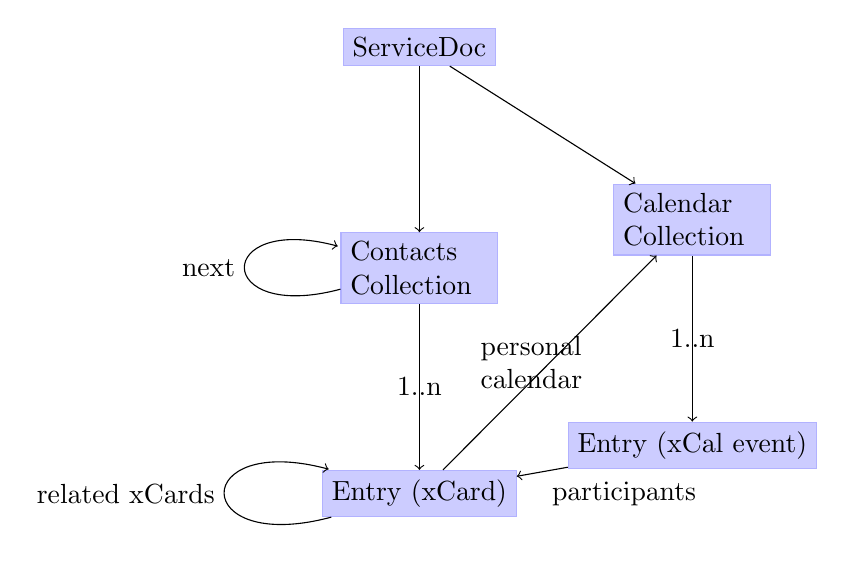
\begin{tikzpicture}
    [doc/.style={rectangle,draw=blue!30,fill=blue!20, node distance=6em}]
    \node[doc] (svc) [] {ServiceDoc};
    \node[doc] (collect) [below=of svc,text width=5em] {Contacts Collection}
      edge [<-] node {} (svc)
      edge [->, loop left] node {next} (collect);

    \node[doc] (calcollect) [below right=of svc,text width=5em] {Calendar Collection}
      edge [<-] node {} (svc);

    \node[doc] (entry) [below=of collect] {Entry (xCard)}
      edge [<-] node {1..n} (collect)
      edge [->] node [text width=5em] {personal calendar} (calcollect)
      edge [->, loop left] node {related xCards} (entry);

    \node[doc] (event) [below=of calcollect] {Entry (xCal event)}
      edge [<-] node {1..n} (calcollect)
      edge [->] node [below right] {participants} (entry);


  \end{tikzpicture}
  \caption{Discovery paths from the Service Document to individual Groupware Resources}
\end{figure}

\subsubsection{Efficient Synchronization with HTTP Delta encoding}

%TODO
TODO

HTTP Delta encoding with Feed:
\citeurl{http://www.wyman.us/main/2004/09/using_rfc3229_w.html}{2012-1-6},
implementations:
\citeurl{http://www.wyman.us/main/2004/09/implementations.html}{2011-1-6}

\subsubsection{Media Entries and the content tag}
\label{sec:inline-feeds-or}

The Atom format provides the opportunity to include a full representation of a
resource in the content tag of an entry\cite[sec. 4.1.3]{RFC4287}. It is thus
possible to embed complete xCard or xCal resources in the Atom feed
and so to relieve the client from issuing many GET requests for each individual
resource.

The benefit of saved GET requests must be balanced with the possible
disadvantage of serving the client resource representations already seen. A
client that does regular updates may probably be interested only in the first
one or two entries of a feed while the server might have made the effort to
produce tens of entries.

On the other hand the Atom Format mandates that an entry without embedded
content must provide a summary element. It may not make much of a difference in
bandwidth and processing whether a summary is produced or the full content is
provided.

Different optimization strategies are possible here, e.g.

\begin{itemize}
\item The first feed in a sequence of paged feeds could contain only very few
  entries to optimize for regular updates and have more entries in all following
  feeds.
\item The server could remember the entries already consumed by an authenticated
  client and serve only new entries in the first feed.
\end{itemize}

In any case it is mandatory that a client can handle embedded content as well as
linked content.

\subsubsection{Modifying Resources}

Editing, Updating and Deleting of media entries is specified in the Atom
Publishing Protocol and is useful for this work without modifications or
additions. Two aspects however are worth to be highlighted.

As outlined in \autoref{sec:inline-feeds-or} it is possible to include full
representations of the collection resources in the content tag of an entry. A
client however is not allowed to use an embedded resource representation as the
base for an update\cite[sec. 10]{RFC5023}. If the client has not yet retrieved
the resource from its own URI it thus `` SHOULD perform a GET on the URI of the
Member Entry before editing it.''[Ibid.] This limitation is consequent since the
Atom feed does not contain an ETag for an embedded resource. A client thus can
not make a conditional PUT request only from the information in the
feed.\footnote{Google adds an etag attribute to the entry tag in its data
  api. \citeurl{http://code.google.com/apis/gdata/docs/2.0/reference.html\#ResourceVersioning}{2012-2-13}}

The second aspect concerns offline editing. A client should offer the user the
possibility to create, update and delete resources while being offline and to
apply this modifications during the next synchronization, much like the IMAP
protocol used by Kolab. This requirement is trivial to fulfill as long as no
concurrent edits happen on the server site. In that case the client needs to
perform an automated or user assisted merge of the conflicting resources. The
client should always preserve a copy of a resource version as last seen from the
Server to be able to perform a three-way-merge.

The problem of offline edits and conflicts is thus similar to the case of a
failed conditional PUT request due to a concurrent edit. \cite{Nielsen1999}
describes this case and resolutions in detail.

\subsubsection{Special Reports, Queries, Search}
\label{sec:spec-reports-search}

In few cases it may not be feasible for a client to synchronize a full
collection, e.g. due to low bandwidth. This section explores restful ways to let
the client request only a subset (selection) of a collection. More specifically
the client should be informed about possible query facilities without relying on
out-of-band information.

A promising approach is to use the de-facto standard
OpenSearch\cite{Clinton}. According to its homepage it is implemented by most
major browsers, search engines and many other sites. OpenSearch is also
recommended for the link type ``search'' in the HTML5
standard\cite[sec. 4.12.4.12]{Hickson2011a}. The default format of an OpenSearch
result list is an Atom (or RSS) feed.

OpenSearch defines the (not yet IANA registered) media type
application/opensearchdescription+xml, which provides necessary information for
a client to perform queries against a search service. Since possible search
queries are usually unlimited it is not possible anymore to provide a set of
static links. Instead the server provides an ``URI Template''\cite{Gregorio2012}
that instructs the client how to perform an ``URI
construction''\footnote{OpenSearch is the older standard and referenced as Level
  1 URI Templates in \cite{Gregorio2012}.}.

The basic OpenSearch standard defines a simple full text search. Thus a user
could search contacts by name, address or any other field value. Equally events,
todo items or notes could be searched by keywords.

The next important use case is to show calendar events in a given interval,
e.g. to present the events for a month, week or day. This can be achieved with
the OpenSearch Time extension that provides the temporal start and end
parameters. Rob Yates CalAtom\cite{draft-yates-atompub-calatom-00.txt} proposal
included a similar time range search as the only but mandatory special report.

Probably useful might be the OpenSocial Geo extension. It could allow to search
contacts or events in a given geographic region. Even more search types become
possible with the SRU extension that wraps the ``Search/Retrieval via URL''
standard with its ``Contextual Query Language''
(CQL)\footnote{\citeurl{http://www.loc.gov/standards/sru}{2012-3-1}}. The latter
provides the possibility to sort result sets which might be interesting to
present an address book sorted by names.

Search result Atom feeds can make use of annotated HTML
(\autoref{sec:microdata}) in the summaries of entries and should not embed full
resources in the content tag. Thus the client can still provide a structured
view of the data, like calendar views or a tabular contacts list without the
need to transfer full representations.

The OpenSearch specification suggests that links to the OpenSearch Description
Document for an Atom feed might be added inside a feed tag. There is however no
reason not to add such a link inside the collection tag of a Service
Document. This allows a client to directly search a collection without the need
to get the feed first.

% \subsubsection{Structural and Behavioral Rest Model}
% @TODO Modelierung der Anwendung mit dem Meta Model nach Schreier.
% Primary Resources: Contacts, Calendars, ...
% List Resources: 

\subsection{Components}

\subsubsection{Dispatcher}
\label{sec:dispatcher}
The dispatcher selects the Java method (see \ref{sec:components-actions}) that
should handle the request. The selection can depend at least on the path
component of the requested URI, the media types accepted by the client as
indicated in the request's ACCEPT header and the HTTP verb.

Every project implementing JAX-RS\cite{JAX-RS1.1} needs to have some kind of
dispatcher component. The specification itself does not identify this
component. It does however specify the algorithm a dispatcher needs to follow
and a set of Java annotations which must be used to configure the
dispatch. These annotations (PATH, GET for the HTTP verb and Produces) are
demonstrated in listing \ref{fig:jaxrs-annotated-resource-example}.

\begin{javalisting}[label=fig:jaxrs-annotated-resource-example,
                   caption={Example of a JAX-RS annotated Resource class (by Marek Potociar)}]
@Path("atm/{cardId}")	
public class AtmResource {	
`  
  @GET 	
  @Path("balance")	
  @Produces("text/plain")	
  public String balance(@PathParam("cardId") String card,	
                        @QueryParam("pin") String pin) {	
    return Double.toString(getBalance(card, pin));	
  }
\end{javalisting}
 
Alternative approaches to configure the dispatcher are not designated by
JAX-RS. One possible alternative would be to expose an API to manually add
dispatch routes at runtime and remove the corresponding annotations from the
source code. 

This approach is indeed implemented e.g. by
Restlet\footnote{\citeurl{http://wiki.restlet.org/docs_2.1/13-restlet/27-restlet/326-restlet.html}{2012-2-6}},
Apache Wink\footnote{called ``Dynamic Resources''
  \citeurl{http://incubator.apache.org/wink/1.1/html/5.1 Registration and
    Configuration.html}{2012-2-7}} and probably others. Jersey 2.0 is also
expected to provide an API for the
dispatcher.\footnote{\citeurl{http://java.net/jira/browse/JERSEY-842}{2012-2-6}}:

Advantages of a dynamic dispatcher configuration would be:

\begin{itemize}
\item The path under which a resource type is served is decoupled from the code
  defining the behavior of the resource. This could enable the reuse of resource
  classes or methods in other contexts.
\item The decision which media types can be consumed or produced may not depend
  solely on the resource class or method. A resource method may work on a domain
  specific data type and the set of supported media types may depend on the
  available converter between media types and the data type. A photo album for example
  resource may be able to consume any number of different image formats that
  a separate component can convert to an internal image representation.
\item The list of supported media types could be created programmatically. This
  enables reuse of set of equivalent media types or combination of media type
  categories for example to combine the sets of image, video and audio media
  types.
\item The concept of resource classes could be replaced altogether. The life
  cycle of a resource class in JAX-RS defaults to the request scope. During one
  request only one resource method is called. Resource methods therefor by
  default don't share state through resource class attributes. It would therefor
  be possible to bind individual functors to dispatcher routes and thus
  composing the equivalent of a resource class at runtime.
\end{itemize}

%@TODO:

The dispatching as defined in JAX-RS does not define any facility for a resource
method to decline its possibility to handle a method at runtime. Such a facility
could either be implemented by a boolean precondition method associated with the
resource method or by a special Exception type that would restart the request
dispatch but this time ignoring the method that threw the exception. If no
alternative request method could be found, the Exception would be propagated and
subsequently transformed into an appropriate error response.

Thus it would be possible to define generic and special purpose request methods
even for cases where the static JAX-RS dispatch algorithm does not provide
sufficient granularity.

While all this flexibility can provide many advantages it has to be kept in mind
how the framework can gather enough knowledge to still help by autogenerating
e.g. WADL documents and responses to HEAD and OPTION requests.

\subsubsection{Resource Facades}
\label{sec:resourcefacades}
Fielding discerns between a resource and the representation of a resource in a
certain format, ``selected dynamically based on the capabilities or desires of
the recipient and the nature of the resource''\cite[p. 87]{Fielding2000}.
According to this notion, the media type used to represent a resource should not
influence the processing logic. In an ideal case all possible media types should
be handled by the same resource method.

% man kann, aber man muss nicht, also warum willst du dann ein problem lösen?
% Außerdem mag eine solche Unterscheidung vllcht manchmal aus technischen
% Gesichtspunkten vielleicht doch Sinn machen, zB wenn ich eine Darstellung
% einer Resource in textueller Form (zB XML) und in visueller (zB ein JPG) habe,
% dann mag vllcht unterschiedliche Behandlung doch mal notwendig bzw sinnvoll
% sein. Außerdem sagt Fielding in Abschnitt 5.2.1.2: "A representation can be
% included in a message and processed by the recipient according to the control
% data of the message and the nature of the media type". D.h. die Verarbeitung
% kann vom Medientyp abhängig sein. Und gerade unter dem Gesichtspunkt, dass du
% untersuchen sollst, wie man verschiedene Medientypen unterstützen kann, ist es
% vllcht nicht gut, eine medientypabhängige Verarbeitung auszuschliessen. Wenn
% möglich will man Codedoppelungen natürlich vermeiden, aber manchmal braucht
% man eben unterschiedlichen Code.

This ideal contrasts with JAX-RS concepts where the media type can be one
parameter of the dispatcher logic. This section outlines a pattern tentatively
named ``Resource Facades'' that should make it easier to handle different media
types with the same code and thus to facilitate code reuse.

% das fällt vom Himmel, es gibt kein Problem, das du bis zu dem Zeitpunkt
% beschrieben hast und beschreibst dann ein Pattern, wo auch nicht klar ist wo
% das her kommt. Wenn du das selber entwickeln willst, musst du erstmal das
% Problem analyisieren und beschreiben und dann kann man ein Pattern
% entwickeln. Vor allem gibt es für Pattern auch gewisse Richtlinien wie man
% diese beschreibt und vielleicht wäre es hilfreich sich daran zu orientieren

A resource method should contain the programming logic executed to serve a
request of a specific type (e.g. GET, PUT) against a specific resource. The
programming logic could execute common tasks like the following:

\begin{itemize}
\item validate the correctness of a submitted resource
\item check the clients authorization
\item persist the submitted resource data
\item trigger notifications containing a summary of the resource
\item submit the submitted resource to an indexing system
\item check the submitted resource to be of a certain accepted domain type, like
  contact, event, todo item or any set of such types
\end{itemize}

All the above processing tasks should in theory be independent of the media type
of a resource and only be programmed once to work on any resource format. This
could be made possible by applying the concept of roles to resources. Roles have
been described already 15 years ago by \cite{Fowler1997} or a bit later by
\cite{Baeumer2000}. However no evidence could be found whether roles have been
used to implement restful systems.

According to \cite{Steimann2008}, there exists several definitions for roles
which mostly share a few core properties:

\begin{quote}
  This includes the property that a single object can play several roles of
  different or the same kind both simultaneously and sequentially, and that the
  same role can be played by different objects of the same and different
  kinds. Raised to the type level, this means that the relationship between role
  types and class types (as sources of role players) is generally m:n.
\end{quote}

A popular example for roles is a person, that can have the different roles over
their lifetime (student, professor, single, husband, widower) or in different
contexts (teacher, father, husband, customer, politician).

% \cite{Steimann2001} repeats the necessity of the dynamic role concept and argues
% that (Java) interfaces serve as an appropriate mean to handle roles.

Exemplified with the above tasks, a resource can have the role of being
validated, persisted, summarized or checked for being of a certain type. So like
in the above quote a facility is needed that can provide m different roles of
resources that come in n different shapes.

It can be noted, that unlike in the previous example with roles of a person,
this resource roles examples do not extend the original resource with new
attributes. A person surely gets additional attributes as a father (references
to children) or professor (member of faculty). Thus the term ``facade'' in favor
of role should indicate that only different views of the same data are provided.

Listing \ref{fig:datafacades-api} shows interfaces of a minimal framework to
provide Facades for Resources. The idea is, that any code that needs information
from a Resource requests the appropriate Facade from the ResourceHandler. The
ResourceHandler was instantiated with a FacadeRegistry from which it can request
Factories for requested Facades. A ResourceHandler must have been instantiated
with at least one initial input Facade, e.g. an InputStream.

\begin{javalisting}[label=fig:datafacades-api,
                    float=p,
                   caption={API of the ResourceFacades component}]
interface FacadeFactory<T> {
 T build(ResourceHandler resourceHandler);

 /**
  * Dependency Facades needed by this factory.
  */
 Iterable<? extends Class<?>> getDependencies();
}

interface FacadeRegistry {
 /**
  * Returns Facade factories that could probably
  * build the requested Facade.
  *
  * @param mediaType MediaType of the original Resource
  * @param clazz requested Facade interface
  */
 Iterable<FacadeFactory<?>> getFacadeFactories(MediaType mediaType,
                                               Class<?> clazz);
}

interface ResourceHandler {
 /**
  * Returns the unique instance of a Facade for this Resource
  *
  * Subsequent calls with the same parameter receive the
  * _same_ unique Facade instance!
  *
  * @param clazz requested Facade interface
  * @return Facade implementation instance
  */
 <T> T getFacade(Class<T> clazz);

 /**
  * Is the requested Facade interface available for this Resource?
  *
  * @param clazz Facade interface
  */
 boolean hasFacade(Class<?> clazz);

 /**
  * The MediaType of the original Resource from which this 
  * ResourceHandler was instantiated.
  */
 MediaType getMediaType();
}
\end{javalisting}

\autoref{fig:facade-ex-dependen} presents two example use cases for Facades. On
the left site the request method might want to know the full name of a submitted
contact resource. It therefor requests a Person facade. Different Person Facade
factories are registered. The different factories in turn have each a dependency
on an InputStream parameterized with a Media Type. The provided Media Type makes
the resolution path unambiguous.

The right site shows dependencies of Title and Summary Facades. Different
Factories would be provided that knows to create meaningful titles and summaries
for Persons, Events or Todo items independent of the original Media Types. A
title of a person surely includes the full name, for an event the date and event
title would be combined and a todo item could include the priority in the title.

\begin{figure}[t]
  \centering
  \subfloat{
  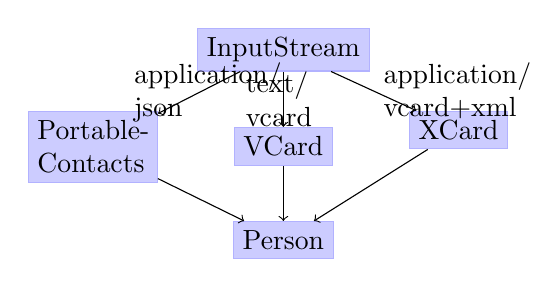
\begin{tikzpicture}
    [doc/.style={rectangle,draw=blue!30,fill=blue!20, node distance=2em}]

    \node[doc] (input) [] {InputStream};
    \node[doc] (poco) [below left=of input,text width=4em] {Portable\-Contacts}
      edge [<-] node [left,text width=2em] {application/ json} (input);

    \node[doc] (vcard) [below=of input] {VCard}
      edge [<-] node [left,text width=1em] {text/ vcard} (input);

    \node[doc] (xcard) [below right=of input] {XCard}
      edge [<-] node [right,text width=3em] {application/ vcard+xml} (input);

    \node[doc] (person) [below=of vcard] {Person}
      edge [<-] node [right] {} (poco)
      edge [<-] node [right] {} (vcard)
      edge [<-] node [right] {} (xcard);
  \end{tikzpicture}  
  }
  \subfloat{
  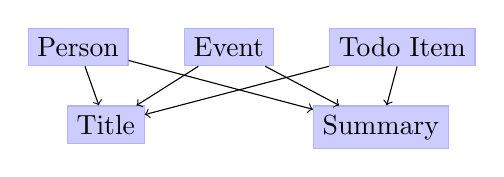
\begin{tikzpicture}
    [doc/.style={rectangle,draw=blue!30,fill=blue!20, node distance=2em}]

    \node[doc] (event) [] {Event};
    \node[doc] (person) [left=of event] {Person};
    \node[doc] (todo) [right=of event] {Todo Item};

    \node[doc] () [below left=of event] {Title}
      edge [<-] node [] {} (todo)
      edge [<-] node [] {} (person)
      edge [<-] node [] {} (event);

    \node[doc] () [below right=of event] {Summary}
      edge [<-] node [] {} (todo)
      edge [<-] node [] {} (person)
      edge [<-] node [] {} (event);
  \end{tikzpicture}
  }
  \caption{Facade examples with dependencies}
  \label{fig:facade-ex-dependen}
\end{figure}


    % Facades provide read-only access to the data
    % Facades can depend on other Facades and thus reuse work
    % Facades could do:
    %     Parse the InputStream with a common JSON/XML framework
    %     Could check whether the data represents a concept like a contact or calendar item, independent from the underlying Media Type (vCard, xCard, portable contacts, iCal, xCal)
    %     Could provide a transformation to another representation (XML<->JSON, xCard to portable contacts)
    %     could extract generic informations from different media types: Title, Authors, Updated, Summary
    % A Facade (Java Interface) that provides access to the Name of a Contact Resource could be implemented by different classes that could work either on vCard, xCard or Portable Contacts. The resource method does not need to be aware or the original media type of the data.

% The concept is powerful because Facades can easily be added without changing
% existing classes. In JAX-RS the resource Method needs to decide, on which
% representation of the data it wants to work. With this concept, a resource
% method could use several different available Facades to access the data.

% Using a similar concept to build representations (request Facades) for different MediaTypes may not be worth the effort.
% This would mostly be necessary to handle GET requests. GET requests however are expected to be idempotent and therefor should contain little to no internal side effects.
% It therefor seems to be reasonable to provide one GET request method for every produced Media Type.
% Specialized get requests may also execute faster than an approach that needs to dynamically build the processing pipeline.

% JAF + REST proposed in 2007 http://www.javaworld.com/javaworld/jw-10-2007/jw-10-resteasy.html

\paragraph{Related work}
\label{sec:resourcefacadesrelated-work}

The idea for the Resource Facades concept was triggered by the use of the
JavaBeans Activation
Framework\footnote{\citeurl{http://www.oracle.com/technetwork/java/javase/downloads/index-135046.html}{2012-2-24}}
(JAF) in the JAX-RS specification. In this framework the DataHandler interface
provides access to available commands for a specific MediaType via the
getCommand method. The framework however was designed with the needs of a
Desktop clipboard in mind. Since JAF has been released for Java version 1.4 it
also does neither support Generics nor uses the advantages of immutability.

\cite{Pradel2008a} presents an approach and implementation in Scala to attach
roles to arbitrary objects. The work achieves type safe roles without extending
the underlying language. Using this library has been considered but it was
discovered too late to be included. Open questions are, how the declared media
type of a Resource could be considered in the selection of a role implementation
and how roles could depend on other roles. Another challenge would be to
preserve role instances and thus to avoid recreating them for every
invocation. If is furthermore required that roles implement a given
interface. The Resource Facade approach presented here is slightly different in
that creation of the facades is implemented independent from the facades
themselves by the factory classes.

JAX-RS provides the MessageBodyReader and -Writer interfaces. However these
interfaces are expected to be used only once per request. The resource method
afterwards needs to work with whatever interface was produced by the
MessageBodyReader. There exists no facility to request additional
transformations or facades of a Resource.

It is possible in JAX-RS to request a MessageBodyReader instance from the
javax.ws.rs.ext.Providers interface. This couldn't however help to get
additional Facades since the InputStream has already been consumed.

The concept shows similarities with Dependency Injection since dependencies of a
facade are also provided by an external component. It may be possible that the
concept could even be implemented on top of an existing Dependency Injection
framework.\footnote{Scala can provide Dependency Injection solely with language
  features via the so called ``Cake
  Pattern''. \citeurl{http://www.warski.org/blog/2011/04/di-in-scala-cake-pattern-pros-cons/}{2012-2-24}
  or Odersky: ``Scalable Component Abstractions''} Some aspects however may
require extra care:

\begin{itemize}
\item Resolving the dependencies of Facade factories must consider the Media
  Type of the input data.
\item The scope of an instance is bound to the ResourceHandler which in most
  cases may be equivalent to the Request scope, but this can't be guaranteed.
\item Each ResourceHandler manages its own view of available Facades.
\end{itemize}

The Apache Wink Rest Framework implements a concept called
``Assets''.\footnote{\citeurl{https://cwiki.apache.org/WINK/59-assets.html}{2012-2-28}}
Assets are containers for the resource data injected in or returned from
resource methods. Assets provide methods annotated with \lstinline:@Produces: or
\lstinline:@Consumes: to handle different Media types. In contrast to Resource
Facades, the set of supported media types of assets can only be extended by
extending the asset classes. It is also not possible like in listing
\ref{fig:facade-ex-dependen} to provide generic Facades for a title or a
summary.

\paragraph{Scala's type system}
The proposed Java class diagram in this section has the disadvantage that the
availability of a facade can not be checked at compile time. It seems however,
that a more advanced type system could help in this regard.

Listing \ref{fig:facades-with-scala-types} demonstrates features of the Scala
type system\cite{Odersky2011} that could be of interest here. In the example a
post method handler has the requirement to access the posted data through the
facades \lstinline:VCard: and \lstinline:TextSummary:. Additionally the data
should be forwarded to an implementation of the trait Storage which has its own
requirement for a facade.

Scala's ``compound types'' feature is used in line \ref{line-scala-compound} to
combine these requirements into an anonymous type. The ``type alias'' feature
allows it to assign the identifier \lstinline:MessageBody: to this anonymous
type and thus to keep the declaration of the \lstinline:post: method short and
readable.

\begin{javalisting}[label=fig:facades-with-scala-types,
                   numbers=left,
                   escapeinside={(*@}{@*)},
                   caption={Implementing the facades approach with Scala's type system}]
trait Storage[ReqFacade] {
 def create(id: String,
            body: ResourceHandler with FacadeFactory[ReqFacade])
}

class PostToCollection[StorageReqFacade]
            (storage: Storage[StorageReqFacade]) {
 type MessageBody = ResourceHandler (*@\label{line-scala-compound}@*)
                      with FacadeFactory[VCard] 
                      with FacadeFactory[TextSummary]
                      with FacadeFactory[StorageReqFacade]
  
 def post(body:MessageBody) : Response = {
  ...
  storage.create("id", body)
  ...
 }
}
\end{javalisting}

This example and the mentioned work on Scala roles shows that an advanced type
systems may be able to considerably improve the presented facades approach. A
more detailed study however is out of the scope of this work and the author's
comprehension of type systems.


\subsection{Producing Semantically annotated HTML}

A recent discussion of possibilities to produce semantically annotated HTML can
be found in \cite[sec. 9.1.3]{DBLP:books/daglib/0023755}. The authors describe a
method developed as part of a larger ``Web Semantics Design Method'' (WSDM),
consists of two mappings. The first one is the ``data source mapping (DSM),
which describes exactly how the reference ontology maps to the actual data
source.''  The second mapping links HTML tags to elements of the reference
ontology from the first mapping. Neither the book nor referenced papers however
go in any more detail about the final step of generating the annotated HTML
tags.

One important point can be learned from the WSDM description. The production of
semantically annotated HTML can become a lot easier if the entity is already
available represented with the targeted vocabulary. A very naive approach to
produce annotated HTML would be to just manually write the necessary attributes
in the template and fill them with values from an arbitrary data object, as
demonstrated in listing \ref{fig:naive-microdata-template}. Even with the
conciseness of the used template language
Jade\footnote{\citeurl{http://scalate.fusesource.org/documentation/jade-syntax.html}{2012-2-22}
  Jade is the most concise among several supported template languages of the
  Scalate Template Engine.}, the developer still has a lot to type.

\begin{anylisting}[label=fig:naive-microdata-template,
                   caption={Defining all Microdata attributes manually in an HTML template}]
-@ var vcard: VCard

div( itemscope itemtype="http://schema.org/Person" 
     itemid=#{vcard.getProperty("uid")} )
  span( itemprop="name" )
    #{vcard.getProperty("fn")}
  span( itemprop="telephone" ) 
    #{vcard.getProperty("tel")}
\end{anylisting}

Compared to the above listing \ref{fig:microdata-template} shows a template
using a data structure that is aware of the used Microdata vocabulary and wraps
an instance of a typed Microdata item with its properties. The
\lstinline:scope: method of the Microdata interface will add the
\lstinline:itemscope:, \lstinline:itemtype: and \lstinline:itemid: attributes to
the nested \lstinline:div: element. The \lstinline:prop: method either augments
a nested element as shown for the \lstinline:name: property or creates the
correct nested element. The method adds the \lstinline:itemprop: attribute and
puts the value for this property inside the element.

\begin{anylisting}[label=fig:microdata-template,
                   caption={Using a Microdata-aware data structure in a template}]
-@ var md: MicroData

= md.scope
  div
    = md.prop("name")
      span( style="color:red" )
    = md.prop("telephone")
    = md.prop("email")
\end{anylisting}

An implementation of this approach must take care of a few
peculiarities\cite{Hickson2011}. Some properties don't necessarily use simple
\lstinline:span: elements, e.g. dates can be better expressed with
\lstinline:time: elements or URI values most likely appear in an
\lstinline:a:, \lstinline:img:, \lstinline:link: or \lstinline:object:
element. Property values could also be put in a \lstinline:content: attribute
while the element's nested text content is optimized for human
consumption. Items can be nested, e.g. an item of type PostalAddress could be
nested inside a Person item.

The proposed approach can be implemented on any template engine as long as it
permits to capture and manipulate nested HTML elements and to call methods of
passed in
objects.\footnote{\citeurl{https://github.com/Paxa/green_monkey}{2012-3-7}
  provides helpers to produce microdata in rails but is not as automated as the
  design proposed here.}

\subsubsection{Other components}

\paragraph{Actions}
\label{sec:components-actions}

An action is basically the code that should be executed to respond to a client
request. An action receives all information about a request and is connected to
the application. It can use and manipulate the application state and produces a
data structure representing the response. It can be compared to the ``Request
method'' defined in JAX-RS.

% With JAX-RS it is not possible to define resource methods in different
% classes, i.e. annotating two different resource classes with the same path.

It is desirable to reuse actions across different consumed media types. Typical
tasks to perform in a POST or PUT resource method are:
\begin{itemize}
\item Transform the input format in a format suitable for the storage component.
\item Check the validity of the received data.
\item Extract information to be sent to another component, e.g. to notify users
  about changes or to index the new data for search.
\end{itemize}

\paragraph{CollectionStorage}
\label{sec:collectionstorage}

The collection storage interface offers the necessary means to store and
retrieve resources. For clarity this interface is not further broken down into a
read-only part and a full read-write interface.

A collection storage is instantiated with the knowledge of the collection it is
responsible for. It therefor typically only returns resources that were
previously stored through it although it may share its underlying persistency
provider with other collection storage instances.

The life cycle of a collection storage is scoped to the application. It is
therefor possible to attach memory based caching to this component.

The storage does not expose any support for transactions. Instead every method
call represents one atomic action independent from other actions. Conditional
request execution is therefor in the responsibility of the storage. Listing
\ref{fig:evaluatepreconditions-concurrency}\footnote{found in the JAX-RS
  specification on page 28.} shows a possibility for a lost update. Another
request could have updated the resource between the etag check and the
\lstinline:doUpdate: call.

\begin{javalisting}[label=fig:evaluatepreconditions-concurrency,
                   caption={Potential lost-update problem with JAX-RS}]
ResponseBuilder rb = request.evaluatePreconditions(etag);
if (rb == null)
  return doUpdate(foo);
\end{javalisting}

% @TODO a resource should not be build, it the etag has not changed. How to make
% etag checking as cheap as possible?

% Contactzilla.com saves portablecontacts json in MongoDB
% https://groups.google.com/d/msg/portablecontacts/57R9gGyoqt0/-P0fF4zRjaoJ

\paragraph{Preparsed Request Components with Dependency Injection}
\label{sec:prep-requ-comp}

It seems like an obvious fact that could not be further deduced, that any
response action to a request must be preluded by a parsing of the request. In
the case of a REST application this parsing could be further divided in two
steps:
\begin{enumerate}
\item Parse URI, Accept Header and HTTP verb to select the Resource method
\item Resource method specific parsing as defined by annotations or done in the
  Resource method
\end{enumerate}

JAX-RS defines only rudimentary support for the second step by means of
inflexible annotations. Listing \ref{fig:jaxrs-annotated-queryparams} shows the
verbosity of parsing a set of standard query parameters for a search
interface. An alternative is shown in listing \ref{fig:request-components}. The
parsing of query parameters is delegated to the class
SearchRequest.\footnote{The QueryParams class is supposed to be an easy
  interface to access query parameters and apply rudimentary validation in one
  step.} The request method ``handleGet'' can access the parameters easily
through the injected SearchRequest instance.

\begin{javalisting}[label=fig:jaxrs-annotated-queryparams,
                   caption={Verbosity of parsing Requests with JAX-RS}]
@Get public Response get(@QueryParam("query") String query,
                         @QueryParam("sort-by") String sortBy,
                         @QueryParam("offset") int offset,
                         @QueryParam("limit") int limit ) {
\end{javalisting}

\begin{javalisting}[label=fig:request-components,
                   caption={Separating Request parsing from the Resource method}]
@GET @Inject
public Response handleGet(SearchRequest sr) { ... }

@RequestScoped
public class SearchRequest {
    public final String query, sortBy;
    public final int offset, limit;
    
    @Inject public SearchRequest(QueryParams qp) {
        query = qp.getNotEmpty("query");
        sortBy = qp.getOrElse("sort-by", "score");
        offset = qp.getPositiveIntOrElse("offset", 0);
        limit = qp.getPositiveIntOrElse("limit", -1);
    }
}
\end{javalisting}

The main advantages of this approach would be:

\begin{itemize}
\item Classes parsing commonly used query parameters can be reused.
\item The request method declaration gets much easier to read.
\item Sophisticated validation can be applied without obfuscating the request method.
\item Default values for unspecified input could depend on information only
  available at runtime instead of being provided as static value to the
  applications source code.
\end{itemize}

This approach is possible to implement for example with the dependency injection
support provided by the Jersey
framework.\footnote{\citeurl{http://codahale.com/what-makes-jersey-interesting-parameter-classes/}{2012-2-5},
  \citeurl{http://codahale.com/what-makes-jersey-interesting-injection-providers/}{2012-2-5}}

\begin{figure}[tbph]
  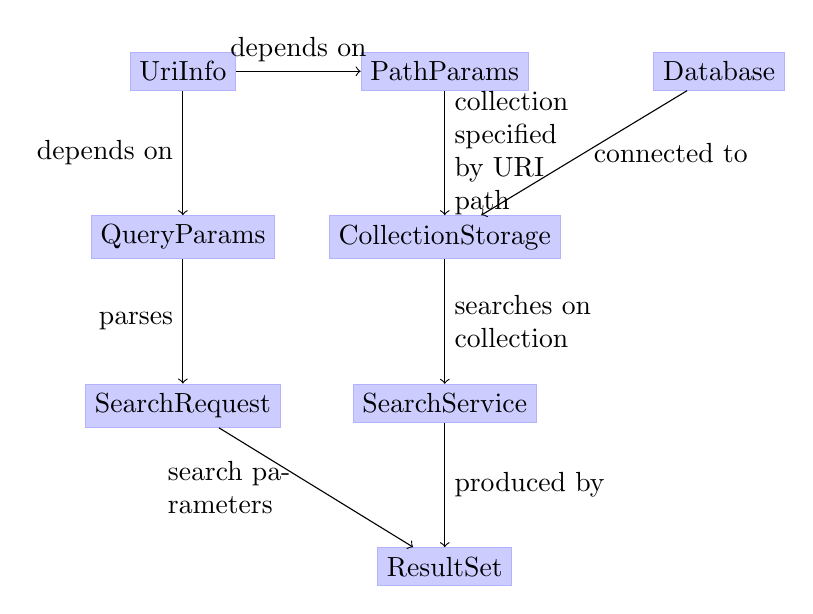
\begin{tikzpicture}
    [doc/.style={rectangle,draw=blue!30,fill=blue!20, node distance=4.5em}]

    \node[doc] (uriinfo) [] {UriInfo};
    \node[doc] (queryparams) [below=of uriinfo] {QueryParams}
      edge [<-] node [left] {depends on} (uriinfo);

    \node[doc] (searchrequest) [below=of queryparams] {SearchRequest}
      edge [<-] node [left] {parses} (queryparams);

    \node[doc] (pathparams) [right=of uriinfo] {PathParams}
      edge [<-] node [above] {depends on} (uriinfo);

    \node[doc] (database) [right=of pathparams] {Database};

    \node[doc] (collection) [below=of pathparams] {CollectionStorage}
      edge [<-] node [right] {connected to} (database)
      edge [<-] node [right,text width=5em] {collection specified by URI path} (pathparams);

    \node[doc] (searchservice) [below=of collection] {SearchService}
      edge [<-] node [right,text width=5em] {searches on collection} (collection);

    \node[doc] (resultset) [below=of searchservice] {ResultSet}
      edge [<-] node [left,text width=5em] {search parameters} (searchrequest)
      edge [<-] node [right] {produced by} (searchservice);
  \end{tikzpicture}
  \caption{Building a processing pipeline with Dependency Injection}
  \label{fig:dependency-injection-pipeline}
\end{figure}

\paragraph{Driving Dependency Injection further}

The use of dependency injection could be extended to comprise several levels of
dependencies and thus to build processing pipelines.  The information from the
above SearchRequest class is probably just forwarded by ``handleGet'' to another
component that executes the search on a given collection. Thus the request
methot is ultimately interested on the search result set to transform it into a
response. Consequently the ``handleGet'' method could use dependency injection
to request the result set and only start working on this. Figure
\ref{fig:dependency-injection-pipeline} visualizes the hypothetic dependency
graph of an application specific ResultSet class.

The figure shows how the CollectionStorage to search on is identified by the URI
path and the search parameters by the SearchRequest class of listing
\ref{fig:request-components}. The dependency injection is configured to produce
a ResultSet class by executing a SearchService with the request scoped
CollectionStorage and SearchRequest.

The idea might be an alternative implementation of processing pipelines to the
one proposed in \cite{Davis:2011:XTR:1967428.1967437}, which uses XProc, An XML
Pipeline Language. One advantage of the dependency injection approach would be
that the processing pipeline can be defined and configured in the same language
then the rest of the application.

%\paragraph{GenericResourceAttributes}
%\label{sec:component-genericresourceattrib}

%\subsection{Detailed Design Considerations}

%\subsection{Client Design}
%What needs a client to know, how does it need to work?

\section{Summary and Conclusions}

\newpage
\bibliography{references}{}
\bibliographystyle{alphadin}
\end{document}

% Local Variables:
% ispell-dictionary: "american"
% eval: (progn (flyspell-mode 1) (outline-minor-mode 1) (goto-address-mode 1) (hide-body))
% End:
%  LocalWords:  RESTful programmatically instantiation hypothetic cacheable
% LocalWords:  Algermissen interoperability representable isomorphism
% LocalWords:  Cacheability
